% Replacement examples only. Not included by date2027.tex.
% Fig. 2: replace the existing fig:npusim_flow environment in 3_related_work.tex.
\begin{figure*}[t]
    \centering
    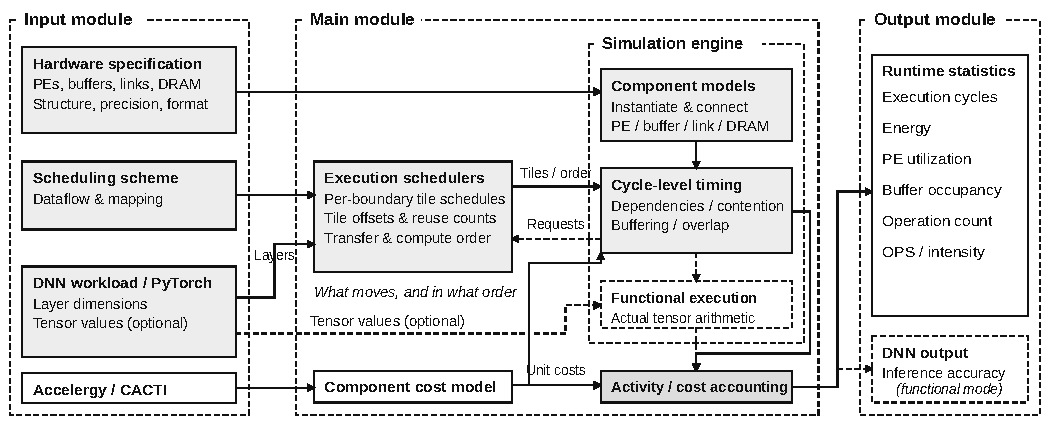
\includegraphics[width=\linewidth]{figures/drafts_v2/fig2_npusim_overview.pdf}
    \caption{Overview of NPUsim. Separate hardware specifications, scheduling schemes, and DNN workloads drive modular hardware models and execution schedulers. Schedulers determine tile transfers and execution order, while hardware models determine cycle costs and component availability. Traced activities and component cost models produce runtime statistics; functional execution optionally evaluates actual tensor values.}
    \label{fig:npusim_flow}
\end{figure*}

% Fig. 3: replace the existing fig:component_library environment in 4_npusim.tex.
\begin{figure}[t]
    \centering
    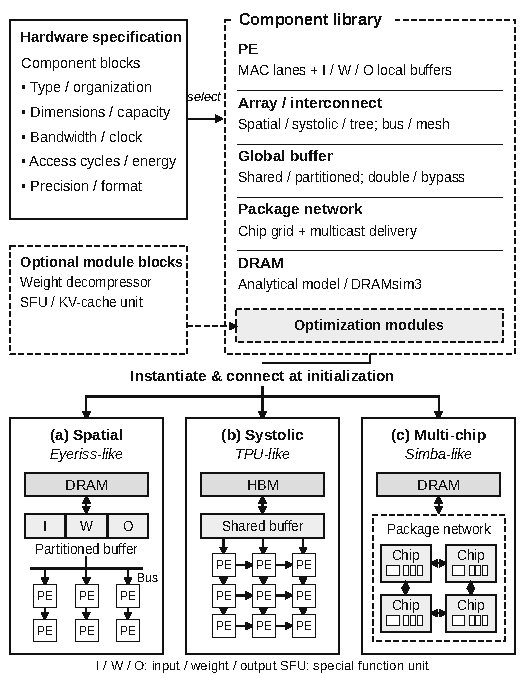
\includegraphics[width=\linewidth]{figures/drafts_v2/fig3_configurable_architecture.pdf}
    \caption{Configurable architecture modeling in NPUsim. Hardware configuration blocks select and parameterize a shared component library, which is instantiated and connected at initialization to compose spatial (Eyeriss-like), systolic (TPU-like), and multi-chip (Simba-like) architectures. Optional configuration blocks enable specialized optimization modules. The depicted array and chip counts are illustrative.}
    \label{fig:component_library}
\end{figure}

% Fig. 4: replace the existing fig:scheduling_and_simulation environment.
% Panel titles already contain (a)/(b); suppress printed subfloat labels
% while retaining subfig counters and the existing cross-reference labels.
\begin{figure*}[t]
    \centering
    \captionsetup[subfloat]{labelformat=empty}
    \subfloat[]{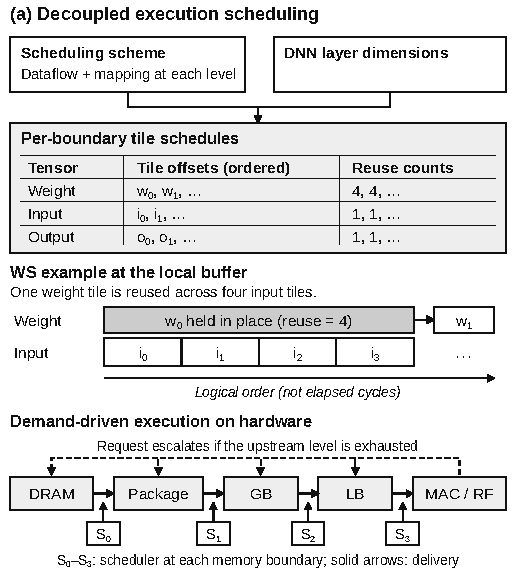
\includegraphics[width=0.4918\linewidth]{figures/drafts_v2/fig4a_execution_scheduling.pdf}\label{subfig:execution_scheduler}}%
    \hfill
    \subfloat[]{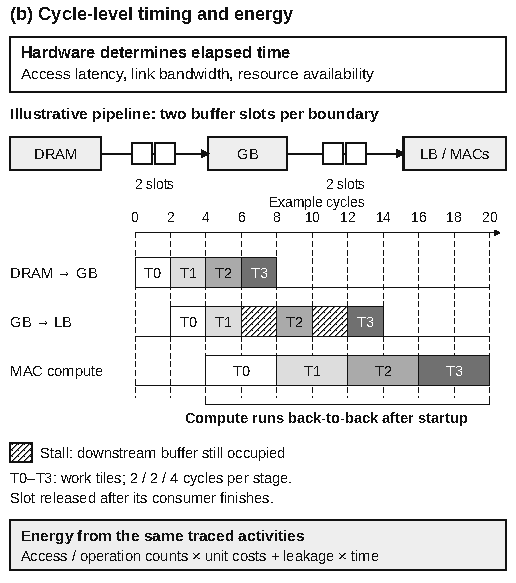
\includegraphics[width=0.4918\linewidth]{figures/drafts_v2/fig4b_timing_energy.pdf}\label{subfig:cycle_level_simulation}}%
    \caption{Decoupled scheduling and cycle-level execution in NPUsim.
    (a) Per-boundary schedulers derive tensor tile offsets and reuse counts from the commanded dataflow and mapping. A weight-stationary example holds one weight tile across four input tiles; runtime requests propagate up the memory hierarchy as needed.
    (b) Hardware costs and buffering compose scheduled work into a cycle-level pipeline. In this illustrative double-buffered example, the compute stage is the bottleneck and upstream transfers stall while local buffer slots remain occupied. The same activities determine energy consumption.}
    \label{fig:scheduling_and_simulation}
\end{figure*}
